    \subsection{Agents and permissions}
        In the following figure (figure \ref{fig:poc-actors}) shows the different agents and it's permissions before the \acrshort{poc}.\\ 
        \begin{figure}[h]
            \centering
            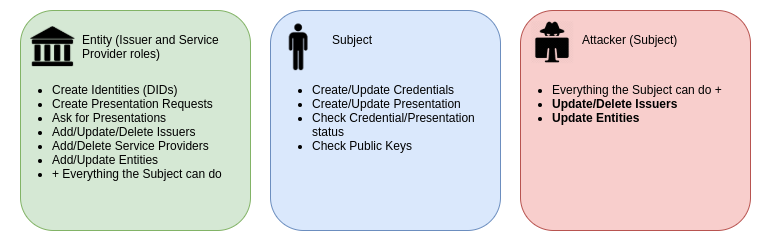
\includegraphics[width=1.0\textwidth]{poc-actors.png}
            \caption{\acrshort{poc} agents and permissions}
            \label{fig:poc-actors}
        \end{figure}
        
        The entity will have the roles of Issuer and Service Provider, but we will only focus on the Issuer role. We will also have an attacker, with the same permissions as a Subject. This means that, the only thing the attacker has is it's own \acrshort{did} (has no more privileges). As we can see, the entity, which can be a bank or a traffic authority, can create Credentials, Presentations, consult public keys and create identities (\acrshort{did}s) among other things. The creation of identities is what interests us in this \acrshort{poc}. We see that the attacker has the ability to delete Issuers, which he should not be able to do. By exploiting this vulnerability, we will stop an entity from being an Issuer, and therefore, from being able to create new identities, as we see graphically in the figure \ref{fig:poc-actors-after}.
        
        \begin{figure}[h]
            \centering
            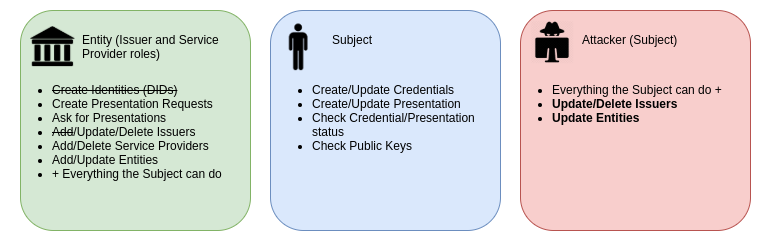
\includegraphics[width=1.1\textwidth]{poc-actors-after.png}
            \caption{\acrshort{poc} agents and permissions after de attack}
            \label{fig:poc-actors-after}
        \end{figure}

